%!TEX root = ../dokumentation.tex

\chapter{Grundlagen} \label{ch:materialsAndMethods}

\textcite{kalyanam_prediction_2016} untersuchen die Auswirkungen von Events in der realen Wert auf die Social Media Aktivität. Ebenso untersuchen \textcite{tsytsarau_dynamics_2014} diesen Zusammenhang, mit einem Fokus auf die Verbindung der medialen Berichterstattung und dem Sentiment, der durch die Social Media Aktivitäten dargestellt wird.
\textcite{gimpel_user_2018} nähern sich der Thematik der Social Media Nutzung durch eine Cluster-Analyse zu verschiedenen Rollen in Twitter-Diskussionen.
Zudem untersucht \textcite{saltzer_bundestagswahl_2022} die Positionen von Bundestagskandidaten auf Twitter und betrachtet diese einerseits im Vergleich innerhalb der Parteien sowie andererseits auf einem allgemeinen politischen Koordinatensystem \autocite{saltzer_bundestagswahl_2022, saltzer_finding_2022}.

\textcite{li_survey_2021} sowie \textcite{kowsari_text_2019} bieten je einen umfassenden Überblick sowie Vor- und Nachteile verschiedener Arten von Text-Klassifikation und gehen dabei sowohl auf traditionelle als auch auf Deep-Learning-Ansätze ein.
\textcite{minaee_deep_2022} untersuchen und vergleichen die Verwendung von Deep-Learning-Modellen für die Aufgabe der Text-Klassifikation.

\textcite{wong_quantifying_2016} bestimmen die politische Ausrichtung aufgrund des Verhaltens von Personen auf Twitter durch die Betrachtung, welche Accounts ähnliche andere Accounts retweeten.
Zudem vergleichen \textcite{doan_using_2022} verschiedene Sprachmodelle zur Klassifizierung von Reden nach Parteien und führen dies für verschiedene Länder bzw. Sprachen durch.
Auch \textcite{biessmann_predicting_2016} klassifizieren Reden nach Parteien und nutzen zum Trainieren Parlaments-Debatten des Bundestages. Zudem wenden sie den Klassifikator auf andere Arten von Texten wie Social Media Posts an.

Die Darstellung der Literatur zeigt, dass sich bereits einige Arbeiten mit der Analyse von Social Media Aktivitäten im Zusammenhang mit realen Events sowie mit dem Problem, Texte nach Parteizugehörigkeit zu klassifizieren, beschäftigen.
In unserer Studienarbeit wollen wir neue Klassifikationsverfahren nutzen und vergleichen, um eine höhere Performance als vergangene Arbeiten zu erreichen.
Zudem wollen wir nicht nur die Texte von Reden nutzen, sondern auch Social Media Posts und Parteiprogramme als Trainingsdaten für den Klassifikator einbeziehen.
Für die darauf aufbauenden Analysen wollen wir zusätzlich zu den Social Media Aktivitäten, die mit bestimmten Ereignissen in Verbindung stehen, auch die jeweilige politische Einstellung der Nutzer, bestimmt durch den trainierten Klassifikator, nutzen.

-   Politikapparat und Parteienlandschaft
-   Erörterung, welche Medienplattformen und Nachrichtenquellen verwendet werden sollen
-   Auswahl von Quellen und Sammeln von Daten
-   NLP-Pipeline
-   Machine Learning / Clustering

\section{Deutsche Politik}
Eine gute Übersicht über die notwendigen politikwissenschaftlichen Hintergründe bieten \textcite{bukow_innerparteiliche_2013}, die die Organisation und Funktion der deutschen Parteien beschreiben.

\subsection{Politischer Bias}

\begin{figure}[H]
    \centering
    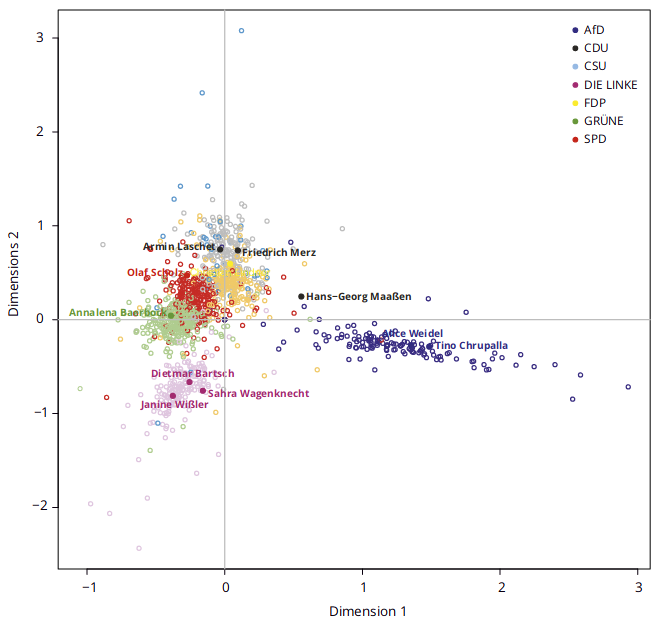
\includegraphics[width=0.5\textwidth]{images/positionierung_ausgewaehlter_kandidaten.png}
    \caption[Positionierung ausgewählter Kandidat:innen]{Positionierung ausgewählter Kandidat:innen innerhalb eines zweidimensionalen politischen Raums \autocite{saltzer_bundestagswahl_2022}} \label{fig:positionierungAusgewaehlterKanidaten}
\end{figure}

\subsection{Aktuelle Regierung im Zeitraum 2017 bis 2021}

\section{NLP}

\subsection{Cleaning Pipeline}

- Common Sense aus der Literatur

\section{Modeling}

\textbf{Bag-of-Words}:

Lorem Ipsum

\textbf{TF-IDF}:

Die Transformation 

\textbf{Check-worthy sentence detection}:

% \begin{figure}[H]
%     \centering
%     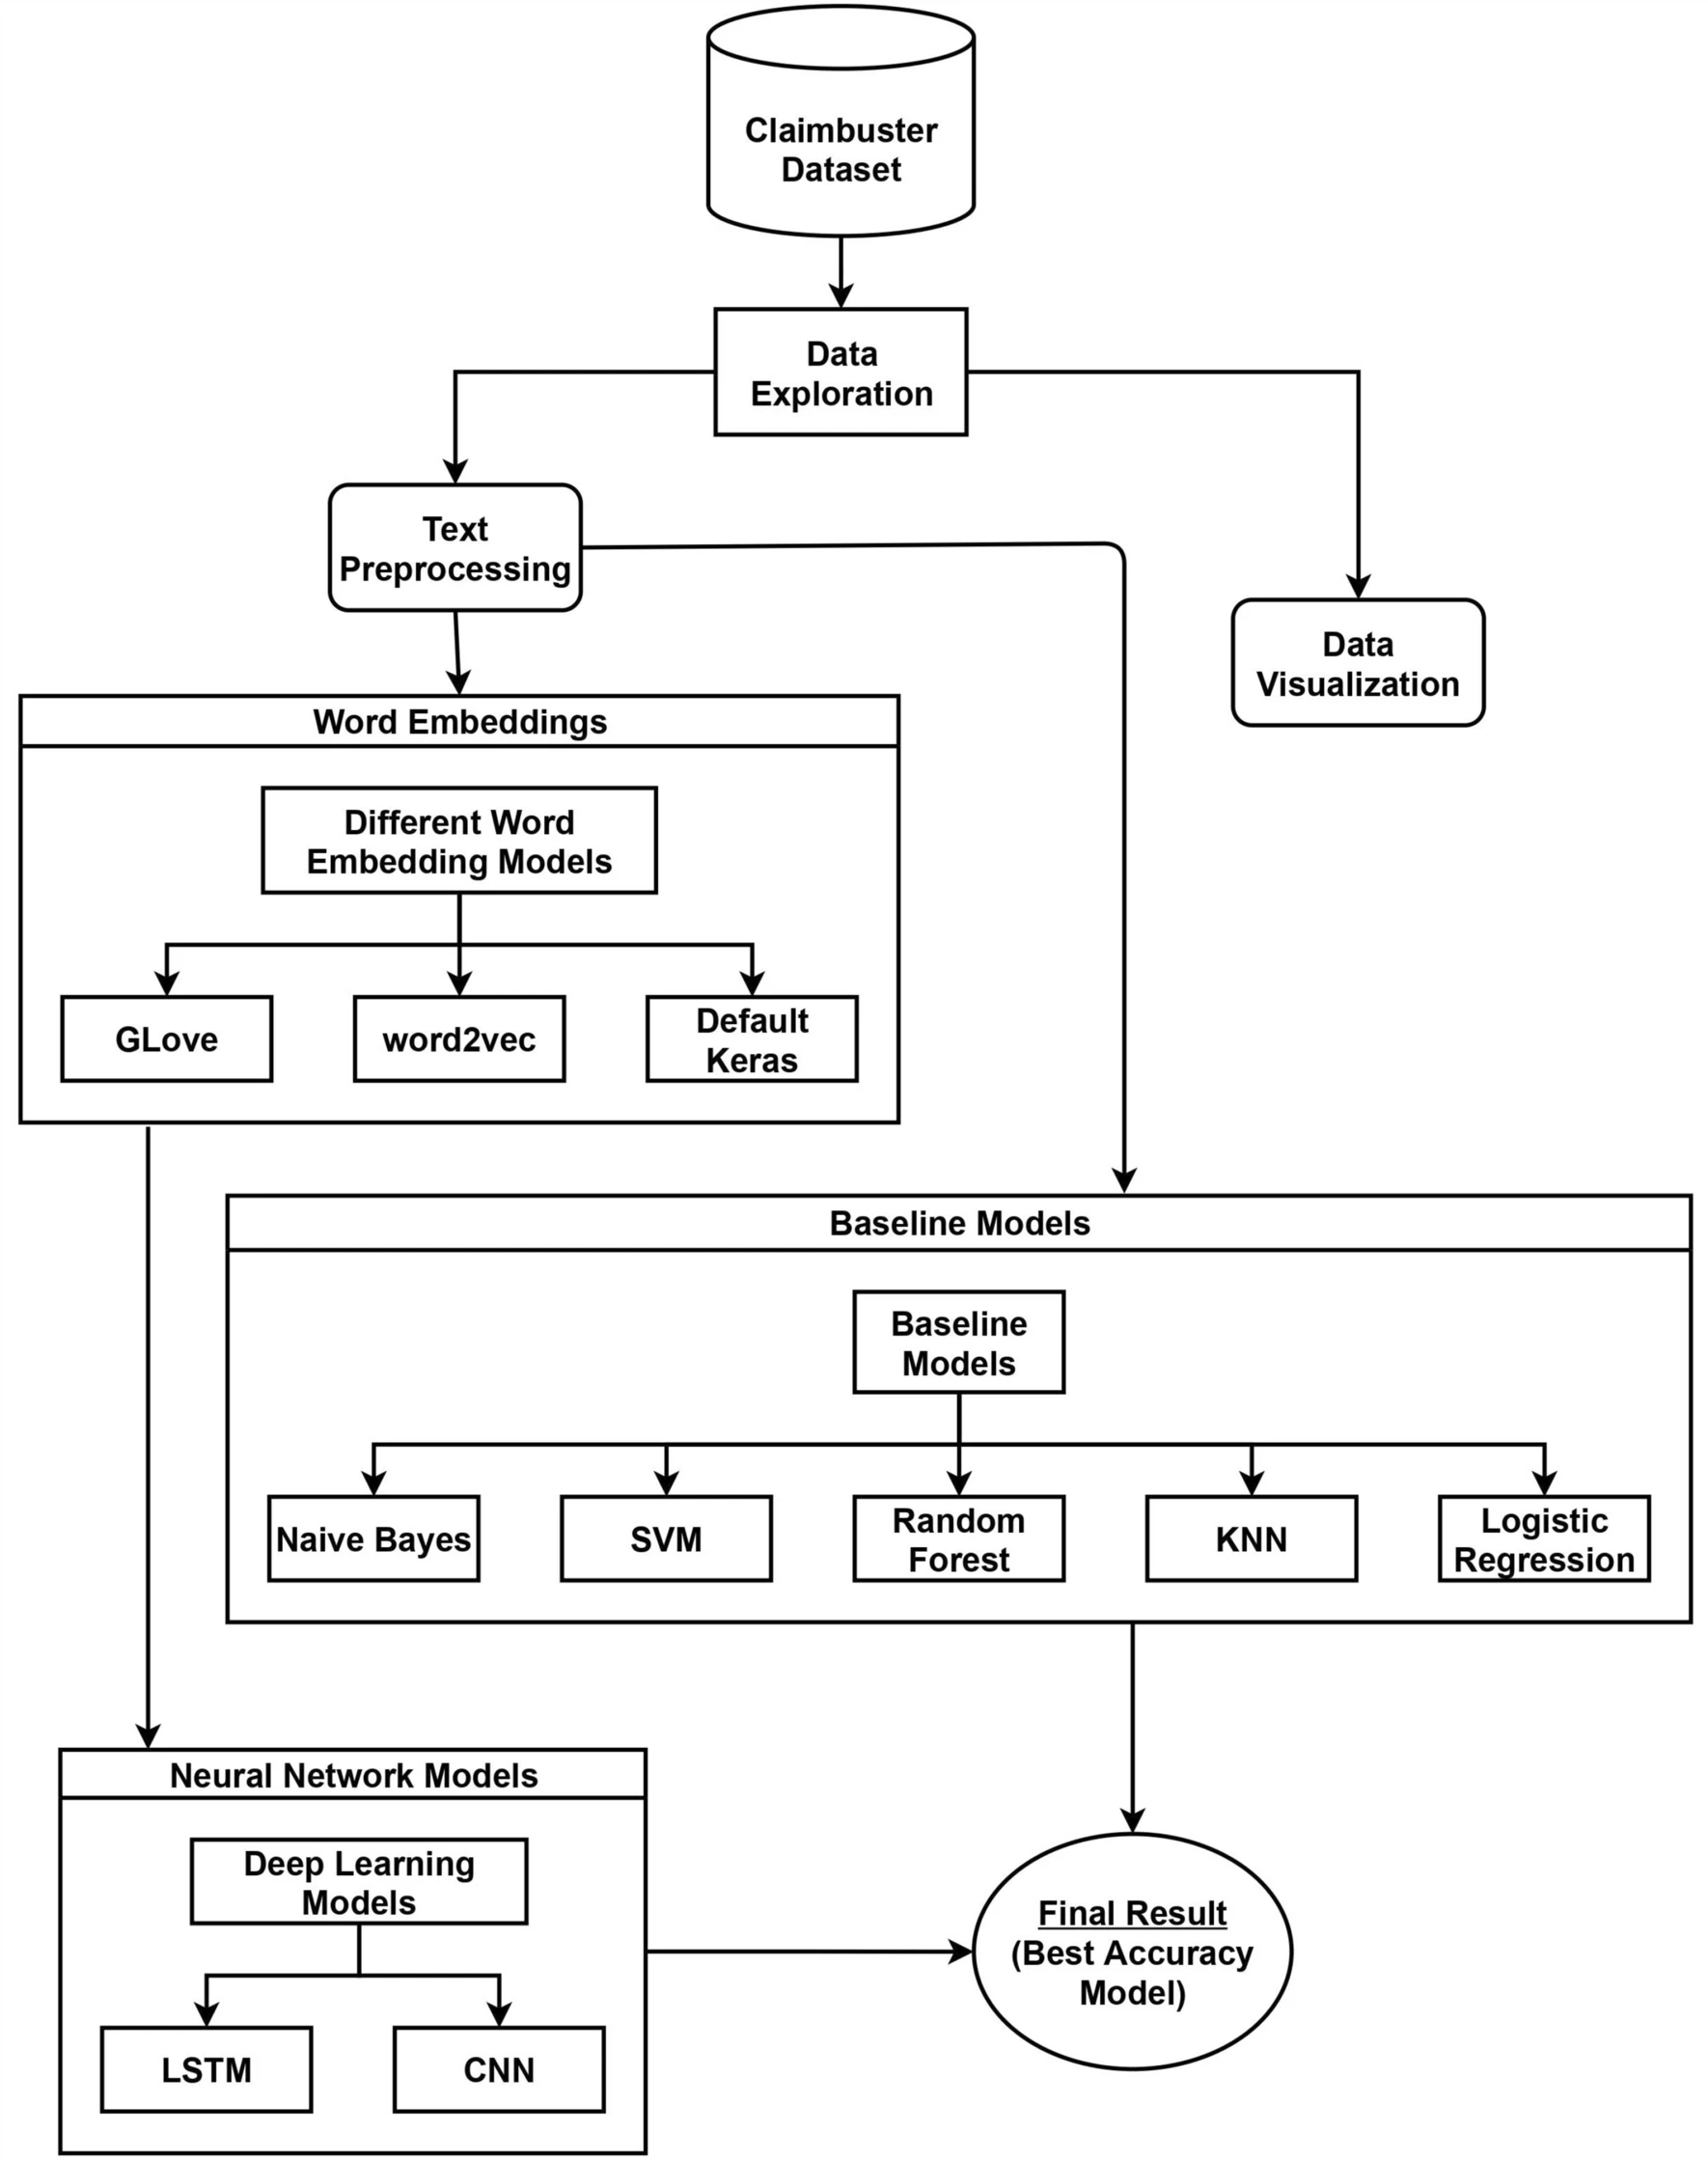
\includegraphics[width=0.8\textwidth]{images/workflow_of_experiment_design.png}
%     \caption[Workflow of Experiment Design]{Workflow of Experiment Design \autocite{jha_towards_2023}} \label{fig:workflowExperimentDesign}
% \end{figure}

Das G2CW Framework von \textcite{jha_towards_2023} ermöglicht es zu prüfen, ob ein englischer Satz einen Fakt enthält. Zusätzlich klassifiziert das Modell, ob dieser Fakt irrelevant ist, oder ob es sich lohnt, die Richtigkeit des Satzes zu überprüfen (F1-Score \num{0.92}).

Für das Training des \ac{ML} Modells werden zwei unterschiedliche Arten von Modellen trainiert. Als Ausgangsmetrik werden herkömmliche Modelle wie Naive Bayes, \ac{SVM} und Random Forest verwendet. Diese werden mit Features aus einzelnen Sätzen und \ac{POS} Features trainiert. Zusätzlich werden Deep Leaarning Modelle wie \ac{LSTM} und \ac{CNN} verwendet. Für das Training von den letzten Modellen verwenden \textcite{jha_towards_2023} Word Embedding Modelle wie GLove, word2vec und Keras.
